\documentclass[twoside]{book}

% Packages required by doxygen
\usepackage{fixltx2e}
\usepackage{calc}
\usepackage{doxygen}
\usepackage[export]{adjustbox} % also loads graphicx
\usepackage{graphicx}
\usepackage[utf8]{inputenc}
\usepackage{makeidx}
\usepackage{multicol}
\usepackage{multirow}
\PassOptionsToPackage{warn}{textcomp}
\usepackage{textcomp}
\usepackage[nointegrals]{wasysym}
\usepackage[table]{xcolor}

% Font selection
\usepackage[T1]{fontenc}
\usepackage[scaled=.90]{helvet}
\usepackage{courier}
\usepackage{amssymb}
\usepackage{sectsty}
\renewcommand{\familydefault}{\sfdefault}
\allsectionsfont{%
  \fontseries{bc}\selectfont%
  \color{darkgray}%
}
\renewcommand{\DoxyLabelFont}{%
  \fontseries{bc}\selectfont%
  \color{darkgray}%
}
\newcommand{\+}{\discretionary{\mbox{\scriptsize$\hookleftarrow$}}{}{}}

% Page & text layout
\usepackage{geometry}
\geometry{%
  a4paper,%
  top=2.5cm,%
  bottom=2.5cm,%
  left=2.5cm,%
  right=2.5cm%
}
\tolerance=750
\hfuzz=15pt
\hbadness=750
\setlength{\emergencystretch}{15pt}
\setlength{\parindent}{0cm}
\setlength{\parskip}{3ex plus 2ex minus 2ex}
\makeatletter
\renewcommand{\paragraph}{%
  \@startsection{paragraph}{4}{0ex}{-1.0ex}{1.0ex}{%
    \normalfont\normalsize\bfseries\SS@parafont%
  }%
}
\renewcommand{\subparagraph}{%
  \@startsection{subparagraph}{5}{0ex}{-1.0ex}{1.0ex}{%
    \normalfont\normalsize\bfseries\SS@subparafont%
  }%
}
\makeatother

% Headers & footers
\usepackage{fancyhdr}
\pagestyle{fancyplain}
\fancyhead[LE]{\fancyplain{}{\bfseries\thepage}}
\fancyhead[CE]{\fancyplain{}{}}
\fancyhead[RE]{\fancyplain{}{\bfseries\leftmark}}
\fancyhead[LO]{\fancyplain{}{\bfseries\rightmark}}
\fancyhead[CO]{\fancyplain{}{}}
\fancyhead[RO]{\fancyplain{}{\bfseries\thepage}}
\fancyfoot[LE]{\fancyplain{}{}}
\fancyfoot[CE]{\fancyplain{}{}}
\fancyfoot[RE]{\fancyplain{}{\bfseries\scriptsize Generated by Doxygen }}
\fancyfoot[LO]{\fancyplain{}{\bfseries\scriptsize Generated by Doxygen }}
\fancyfoot[CO]{\fancyplain{}{}}
\fancyfoot[RO]{\fancyplain{}{}}
\renewcommand{\footrulewidth}{0.4pt}
\renewcommand{\chaptermark}[1]{%
  \markboth{#1}{}%
}
\renewcommand{\sectionmark}[1]{%
  \markright{\thesection\ #1}%
}

% Indices & bibliography
\usepackage{natbib}
\usepackage[titles]{tocloft}
\setcounter{tocdepth}{3}
\setcounter{secnumdepth}{5}
\makeindex

% Hyperlinks (required, but should be loaded last)
\usepackage{ifpdf}
\ifpdf
  \usepackage[pdftex,pagebackref=true]{hyperref}
\else
  \usepackage[ps2pdf,pagebackref=true]{hyperref}
\fi
\hypersetup{%
  colorlinks=true,%
  linkcolor=blue,%
  citecolor=blue,%
  unicode%
}

% Custom commands
\newcommand{\clearemptydoublepage}{%
  \newpage{\pagestyle{empty}\cleardoublepage}%
}

\usepackage{caption}
\captionsetup{labelsep=space,justification=centering,font={bf},singlelinecheck=off,skip=4pt,position=top}

%===== C O N T E N T S =====

\begin{document}

% Titlepage & ToC
\hypersetup{pageanchor=false,
             bookmarksnumbered=true,
             pdfencoding=unicode
            }
\pagenumbering{alph}
\begin{titlepage}
\vspace*{7cm}
\begin{center}%
{\Large S\+GA TI }\\
\vspace*{1cm}
{\large Generated by Doxygen 1.8.13}\\
\end{center}
\end{titlepage}
\clearemptydoublepage
\pagenumbering{roman}
\tableofcontents
\clearemptydoublepage
\pagenumbering{arabic}
\hypersetup{pageanchor=true}

%--- Begin generated contents ---
\chapter{Namespace Index}
\section{Packages}
Here are the packages with brief descriptions (if available)\+:\begin{DoxyCompactList}
\item\contentsline{section}{\hyperlink{namespace_s_g_a}{S\+GA} }{\pageref{namespace_s_g_a}}{}
\item\contentsline{section}{\hyperlink{namespace_s_g_a_1_1_models}{S\+G\+A.\+Models} }{\pageref{namespace_s_g_a_1_1_models}}{}
\item\contentsline{section}{\hyperlink{namespace_s_g_a_1_1_models_1_1_web_service}{S\+G\+A.\+Models.\+Web\+Service} }{\pageref{namespace_s_g_a_1_1_models_1_1_web_service}}{}
\end{DoxyCompactList}

\chapter{Hierarchical Index}
\section{Class Hierarchy}
This inheritance list is sorted roughly, but not completely, alphabetically\+:\begin{DoxyCompactList}
\item Http\+Application\begin{DoxyCompactList}
\item \contentsline{section}{S\+G\+A.\+Global}{\pageref{class_s_g_a_1_1_global}}{}
\end{DoxyCompactList}
\item Web\+Service\begin{DoxyCompactList}
\item \contentsline{section}{S\+G\+A.\+Models.\+Web\+Service.\+Web\+Service\+S\+GA}{\pageref{class_s_g_a_1_1_models_1_1_web_service_1_1_web_service_s_g_a}}{}
\end{DoxyCompactList}
\end{DoxyCompactList}

\chapter{Class Index}
\section{Class List}
Here are the classes, structs, unions and interfaces with brief descriptions\+:\begin{DoxyCompactList}
\item\contentsline{section}{\hyperlink{class_s_g_a_1_1_global}{S\+G\+A.\+Global} }{\pageref{class_s_g_a_1_1_global}}{}
\item\contentsline{section}{\hyperlink{class_s_g_a_1_1_models_1_1_web_service_1_1_web_service_s_g_a}{S\+G\+A.\+Models.\+Web\+Service.\+Web\+Service\+S\+GA} \\*Summary description for \hyperlink{class_s_g_a_1_1_models_1_1_web_service_1_1_web_service_s_g_a}{Web\+Service\+S\+GA} }{\pageref{class_s_g_a_1_1_models_1_1_web_service_1_1_web_service_s_g_a}}{}
\end{DoxyCompactList}

\chapter{File Index}
\section{File List}
Here is a list of all files with brief descriptions\+:\begin{DoxyCompactList}
\item\contentsline{section}{\hyperlink{_global_8asax_8cs}{Global.\+asax.\+cs} }{\pageref{_global_8asax_8cs}}{}
\item\contentsline{section}{\hyperlink{_web_service_s_g_a_8asmx_8cs}{Web\+Service\+S\+G\+A.\+asmx.\+cs} }{\pageref{_web_service_s_g_a_8asmx_8cs}}{}
\end{DoxyCompactList}

\chapter{Namespace Documentation}
\hypertarget{namespace_s_g_a}{}\section{S\+GA Namespace Reference}
\label{namespace_s_g_a}\index{S\+GA@{S\+GA}}
\subsection*{Namespaces}
\begin{DoxyCompactItemize}
\item 
namespace \hyperlink{namespace_s_g_a_1_1_models}{Models}
\end{DoxyCompactItemize}
\subsection*{Classes}
\begin{DoxyCompactItemize}
\item 
class \hyperlink{class_s_g_a_1_1_global}{Global}
\end{DoxyCompactItemize}

\hypertarget{namespace_s_g_a_1_1_models}{}\section{S\+G\+A.\+Models Namespace Reference}
\label{namespace_s_g_a_1_1_models}\index{S\+G\+A.\+Models@{S\+G\+A.\+Models}}
\subsection*{Namespaces}
\begin{DoxyCompactItemize}
\item 
namespace \hyperlink{namespace_s_g_a_1_1_models_1_1_web_service}{Web\+Service}
\end{DoxyCompactItemize}

\hypertarget{namespace_s_g_a_1_1_models_1_1_web_service}{}\section{S\+G\+A.\+Models.\+Web\+Service Namespace Reference}
\label{namespace_s_g_a_1_1_models_1_1_web_service}\index{S\+G\+A.\+Models.\+Web\+Service@{S\+G\+A.\+Models.\+Web\+Service}}
\subsection*{Classes}
\begin{DoxyCompactItemize}
\item 
class \hyperlink{class_s_g_a_1_1_models_1_1_web_service_1_1_web_service_s_g_a}{Web\+Service\+S\+GA}
\begin{DoxyCompactList}\small\item\em Summary description for \hyperlink{class_s_g_a_1_1_models_1_1_web_service_1_1_web_service_s_g_a}{Web\+Service\+S\+GA} \end{DoxyCompactList}\end{DoxyCompactItemize}

\chapter{Class Documentation}
\hypertarget{class_s_g_a_1_1_global}{}\section{S\+G\+A.\+Global Class Reference}
\label{class_s_g_a_1_1_global}\index{S\+G\+A.\+Global@{S\+G\+A.\+Global}}
Inheritance diagram for S\+G\+A.\+Global\+:\begin{figure}[H]
\begin{center}
\leavevmode
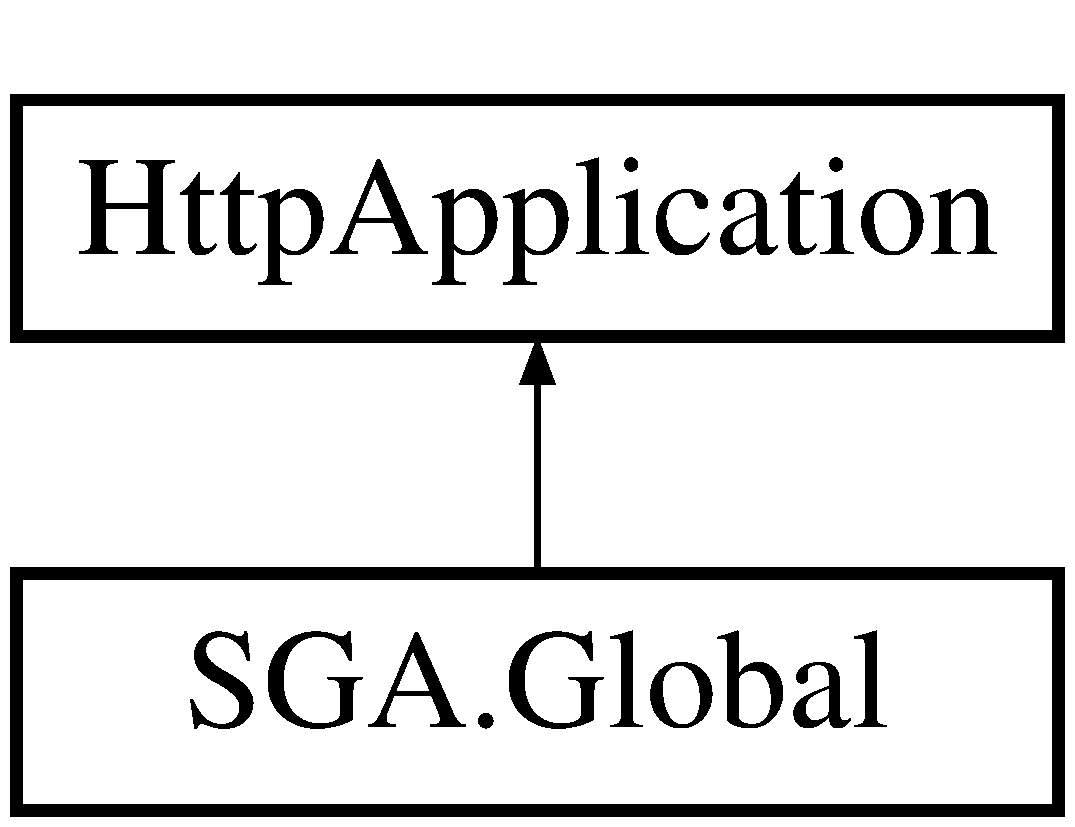
\includegraphics[height=2.000000cm]{class_s_g_a_1_1_global}
\end{center}
\end{figure}
\subsection*{Protected Member Functions}
\begin{DoxyCompactItemize}
\item 
void \hyperlink{class_s_g_a_1_1_global_a91c216f957f9c57c1e11c84c63bbfe4b}{Application\+\_\+\+Start} (object sender, Event\+Args e)
\end{DoxyCompactItemize}


\subsection{Member Function Documentation}
\mbox{\Hypertarget{class_s_g_a_1_1_global_a91c216f957f9c57c1e11c84c63bbfe4b}\label{class_s_g_a_1_1_global_a91c216f957f9c57c1e11c84c63bbfe4b}} 
\index{S\+G\+A\+::\+Global@{S\+G\+A\+::\+Global}!Application\+\_\+\+Start@{Application\+\_\+\+Start}}
\index{Application\+\_\+\+Start@{Application\+\_\+\+Start}!S\+G\+A\+::\+Global@{S\+G\+A\+::\+Global}}
\subsubsection{\texorpdfstring{Application\+\_\+\+Start()}{Application\_Start()}}
{\footnotesize\ttfamily void S\+G\+A.\+Global.\+Application\+\_\+\+Start (\begin{DoxyParamCaption}\item[{object}]{sender,  }\item[{Event\+Args}]{e }\end{DoxyParamCaption})\hspace{0.3cm}{\ttfamily [protected]}}



The documentation for this class was generated from the following file\+:\begin{DoxyCompactItemize}
\item 
\hyperlink{_global_8asax_8cs}{Global.\+asax.\+cs}\end{DoxyCompactItemize}

\hypertarget{class_s_g_a_1_1_models_1_1_web_service_1_1_web_service_s_g_a}{}\section{S\+G\+A.\+Models.\+Web\+Service.\+Web\+Service\+S\+GA Class Reference}
\label{class_s_g_a_1_1_models_1_1_web_service_1_1_web_service_s_g_a}\index{S\+G\+A.\+Models.\+Web\+Service.\+Web\+Service\+S\+GA@{S\+G\+A.\+Models.\+Web\+Service.\+Web\+Service\+S\+GA}}


Summary description for \hyperlink{class_s_g_a_1_1_models_1_1_web_service_1_1_web_service_s_g_a}{Web\+Service\+S\+GA}  


Inheritance diagram for S\+G\+A.\+Models.\+Web\+Service.\+Web\+Service\+S\+GA\+:\begin{figure}[H]
\begin{center}
\leavevmode
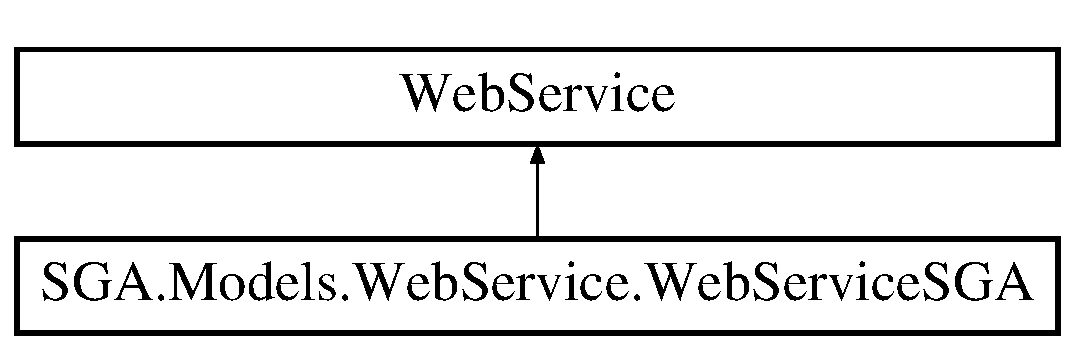
\includegraphics[height=2.000000cm]{class_s_g_a_1_1_models_1_1_web_service_1_1_web_service_s_g_a}
\end{center}
\end{figure}
\subsection*{Public Member Functions}
\begin{DoxyCompactItemize}
\item 
string \hyperlink{class_s_g_a_1_1_models_1_1_web_service_1_1_web_service_s_g_a_a77fc1c1ff075b21635d70b7fe995d623}{Login} ()
\end{DoxyCompactItemize}


\subsection{Detailed Description}
Summary description for \hyperlink{class_s_g_a_1_1_models_1_1_web_service_1_1_web_service_s_g_a}{Web\+Service\+S\+GA} 



\subsection{Member Function Documentation}
\mbox{\Hypertarget{class_s_g_a_1_1_models_1_1_web_service_1_1_web_service_s_g_a_a77fc1c1ff075b21635d70b7fe995d623}\label{class_s_g_a_1_1_models_1_1_web_service_1_1_web_service_s_g_a_a77fc1c1ff075b21635d70b7fe995d623}} 
\index{S\+G\+A\+::\+Models\+::\+Web\+Service\+::\+Web\+Service\+S\+GA@{S\+G\+A\+::\+Models\+::\+Web\+Service\+::\+Web\+Service\+S\+GA}!Login@{Login}}
\index{Login@{Login}!S\+G\+A\+::\+Models\+::\+Web\+Service\+::\+Web\+Service\+S\+GA@{S\+G\+A\+::\+Models\+::\+Web\+Service\+::\+Web\+Service\+S\+GA}}
\subsubsection{\texorpdfstring{Login()}{Login()}}
{\footnotesize\ttfamily string S\+G\+A.\+Models.\+Web\+Service.\+Web\+Service\+S\+G\+A.\+Login (\begin{DoxyParamCaption}{ }\end{DoxyParamCaption})}



The documentation for this class was generated from the following file\+:\begin{DoxyCompactItemize}
\item 
\hyperlink{_web_service_s_g_a_8asmx_8cs}{Web\+Service\+S\+G\+A.\+asmx.\+cs}\end{DoxyCompactItemize}

\chapter{File Documentation}
\hypertarget{_global_8asax_8cs}{}\section{Global.\+asax.\+cs File Reference}
\label{_global_8asax_8cs}\index{Global.\+asax.\+cs@{Global.\+asax.\+cs}}
\subsection*{Classes}
\begin{DoxyCompactItemize}
\item 
class \hyperlink{class_s_g_a_1_1_global}{S\+G\+A.\+Global}
\end{DoxyCompactItemize}
\subsection*{Namespaces}
\begin{DoxyCompactItemize}
\item 
namespace \hyperlink{namespace_s_g_a}{S\+GA}
\end{DoxyCompactItemize}

\hypertarget{_web_service_s_g_a_8asmx_8cs}{}\section{Web\+Service\+S\+G\+A.\+asmx.\+cs File Reference}
\label{_web_service_s_g_a_8asmx_8cs}\index{Web\+Service\+S\+G\+A.\+asmx.\+cs@{Web\+Service\+S\+G\+A.\+asmx.\+cs}}
\subsection*{Classes}
\begin{DoxyCompactItemize}
\item 
class \hyperlink{class_s_g_a_1_1_models_1_1_web_service_1_1_web_service_s_g_a}{S\+G\+A.\+Models.\+Web\+Service.\+Web\+Service\+S\+GA}
\begin{DoxyCompactList}\small\item\em Summary description for \hyperlink{class_s_g_a_1_1_models_1_1_web_service_1_1_web_service_s_g_a}{Web\+Service\+S\+GA} \end{DoxyCompactList}\end{DoxyCompactItemize}
\subsection*{Namespaces}
\begin{DoxyCompactItemize}
\item 
namespace \hyperlink{namespace_s_g_a_1_1_models_1_1_web_service}{S\+G\+A.\+Models.\+Web\+Service}
\end{DoxyCompactItemize}

%--- End generated contents ---

% Index
\backmatter
\newpage
\phantomsection
\clearemptydoublepage
\addcontentsline{toc}{chapter}{Index}
\printindex

\end{document}
